\fancyhead[L]{\textsf{\textbf{MỤC 1.5}}\quad \textsf{Hàm số ngược và Logarit}}
\fancyhead[R]{\textsf{\textbf{65}}}

\noindent
\begin{minipage}[t]{0.485\textwidth}
\fontsize{8.8pt}{11pt}\selectfont
\noindent
\textbf{22.} Trong thuyết tương đối, khối lượng của một hạt chuyển động với vận tốc $v$ là
\[
\setlength{\abovedisplayskip}{3pt}
\setlength{\belowdisplayskip}{3pt}
m = f(v) = \frac{m_0}{\sqrt{1 - v^2/c^2}}
\]
trong đó $m_0$ là khối lượng nghỉ của hạt và $c$ là tốc độ ánh sáng trong chân không. Hãy tìm hàm số ngược của $f$ và giải thích ý nghĩa của nó.

\vspace{1.2ex}
\noindent
\textbf{\textsf{\color{stewartcyan}23--30}} Tìm công thức xác định hàm số ngược của mỗi hàm số sau.

\vspace{0.4ex}
\noindent
\begin{tabularx}{\linewidth}{@{}X X@{}}
\textbf{23.} $f(x) = 1 - x^2,\quad x \geqslant 0$ & \textbf{24.} $g(x) = x^2 - 2x,\quad x \geqslant 1$ \\[1.2ex]
\textbf{25.} $g(x) = 2 + \sqrt{x+1}$ & \textbf{26.} $h(x) = \dfrac{6-3x}{5x+7}$ \\[1.8ex]
\textbf{27.} $y = e^{1-x}$ & \textbf{28.} $y = 3\ln(x-2)$ \\[1.2ex]
\textbf{29.} $y = (2 + \sqrt[3]{x})^5$ & \textbf{30.} $y = \dfrac{1 - e^{-x}}{1 + e^{-x}}$
\end{tabularx}

\vspace{1.2ex}
\noindent
{\color{stewartcyan}\faDesktop}\; \textbf{\textsf{\color{stewartcyan}31--32}} Tìm một công thức tường minh cho $f^{-1}$ và sử dụng nó để vẽ đồ thị của $f^{-1}$, $f$ cùng đường thẳng $y = x$ trên cùng một màn hình. Để kiểm tra lại, hãy xem liệu đồ thị của $f$ và $f^{-1}$ có đối xứng với nhau qua đường thẳng đó hay không.

\vspace{0.6ex}
\noindent
\begin{tabularx}{\linewidth}{@{}X X@{}}
\textbf{31.} $f(x) = \sqrt{4x+3}$ & \textbf{32.} $f(x) = 1 + e^{-x}$
\end{tabularx}

\vspace{1.2ex}
\noindent
\textbf{\textsf{\color{stewartcyan}33--34}} Sử dụng đồ thị đã cho của $f$ để phác thảo đồ thị của $f^{-1}$.

\vspace{0.6ex}
\noindent
\begin{minipage}[t]{0.48\linewidth}
    \textbf{33.}\\[-0.5ex]
    \null\hfill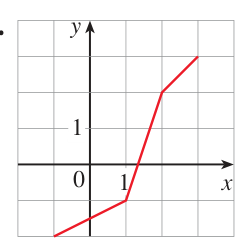
\includegraphics[width=0.76\linewidth]{images/p0100_fig1.png}\hfill\null
\end{minipage}\hfill
\begin{minipage}[t]{0.48\linewidth}
    \textbf{34.}\\[-0.5ex]
    \null\hfill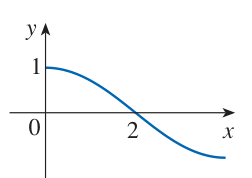
\includegraphics[width=0.86\linewidth]{images/p0100_fig2.png}\hfill\null
\end{minipage}

\vspace{1.2ex}
\noindent
\textbf{35.} Cho hàm số $f(x) = \sqrt{1 - x^2},\ 0 \leqslant x \leqslant 1$.
\begin{enumerate}[label=(\alph*), leftmargin=1.5em, itemsep=0.1ex, topsep=0.3ex, parsep=0pt, partopsep=0pt]
    \item Tìm $f^{-1}$. Hàm số này có mối quan hệ gì với $f$?
    \item Nhận dạng hình học đồ thị của $f$ và giải thích kết quả tìm được ở phần (a).
\end{enumerate}

\vspace{1.2ex}
\noindent
\textbf{36.} Cho hàm số $g(x) = \sqrt[3]{1 - x^3}$.
\begin{enumerate}[label=(\alph*), leftmargin=1.5em, itemsep=0.1ex, topsep=0.3ex, parsep=0pt, partopsep=0pt]
    \item Tìm $g^{-1}$. Hàm số này có liên hệ gì với $g$?
    \item[{\color{stewartcyan}\faDesktop}\; (b)] Vẽ đồ thị của $g$. Bạn giải thích thế nào về kết quả thu được ở phần (a)?
\end{enumerate}

\vspace{1.2ex}
\noindent
\textbf{37.} (a) Hàm số logarit $y = \log_b x$ được định nghĩa như thế nào?
\begin{enumerate}[label=(\alph*), leftmargin=1.5em, itemsep=0.1ex, topsep=0.1ex, parsep=0pt, partopsep=0pt, start=2]
    \item Tập xác định của hàm số này là gì?
    \item Tập giá trị của hàm số này là gì?
    \item Phác thảo dạng đồ thị tổng quát của hàm số $y = \log_b x$ nếu $b > 1$.
\end{enumerate}

\vspace{1.2ex}
\noindent
\textbf{38.} (a) Logarit tự nhiên là gì?
\begin{enumerate}[label=(\alph*), leftmargin=1.5em, itemsep=0.1ex, topsep=0.1ex, parsep=0pt, partopsep=0pt, start=2]
    \item Logarit thập phân là gì?
    \item Phác thảo đồ thị của hàm logarit tự nhiên và hàm mũ tự nhiên trên cùng một hệ trục tọa độ.
\end{enumerate}
\end{minipage}%
\hfill
\begin{minipage}[t]{0.485\textwidth}
\fontsize{8.8pt}{11pt}\selectfont
\noindent
\textbf{\textsf{\color{stewartcyan}39--42}} Tính giá trị chính xác của mỗi biểu thức sau.

\vspace{0.4ex}
\noindent
\textbf{39.} (a) $\log_3 81$ \hfill (b) $\log_3\left(\dfrac{1}{81}\right)$ \hfill (c) $\log_9 3$\hspace*{2em}

\vspace{0.6ex}
\noindent
\textbf{40.} (a) $\ln \left(\dfrac{1}{e^2}\right)$ \hfill (b) $\ln\sqrt{e}$ \hfill (c) $\ln(\ln e^{e^{50}})$\hspace*{0.5em}

\vspace{0.6ex}
\noindent
\textbf{41.} (a) $\log_2 30 - \log_2 15$ \\[0.2ex]
\phantom{\textbf{41.} }(b) $\log_3 10 - \log_3 5 - \log_3 18$ \\[0.2ex]
\phantom{\textbf{41.} }(c) $2\log_5 100 - 4\log_5 50$

\vspace{0.6ex}
\noindent
\textbf{42.} (a) $e^{3\ln 2}$ \hfill (b) $e^{-2\ln 5}$ \hfill (c) $e^{\ln(\ln e^3)}$\hspace*{1.8em}

\vspace{1.2ex}
\noindent
\textbf{\textsf{\color{stewartcyan}43--44}} Sử dụng các quy tắc của logarit để khai triển mỗi biểu thức sau.

\vspace{0.4ex}
\noindent
\textbf{43.} (a) $\log_{10}(x^2 y^3 z)$ \hfill (b) $\ln\left(\dfrac{x^4}{\sqrt{x^2 - 4}}\right)$\hspace*{2em}

\vspace{0.8ex}
\noindent
\textbf{44.} (a) $\ln\sqrt{\dfrac{3x}{x-3}}$ \hfill (b) $\log_2\left[(x^3+1)\sqrt[3]{(x-3)^2}\right]$

\vspace{1.2ex}
\noindent
\textbf{\textsf{\color{stewartcyan}45--46}} Rút gọn biểu thức về dạng một logarit duy nhất.

\vspace{0.4ex}
\noindent
\textbf{45.} (a) $\log_{10} 20 - \frac{1}{3}\log_{10} 1000$ \hfill (b) $\ln a - 2\ln b + 3\ln c$

\vspace{0.6ex}
\noindent
\textbf{46.} (a) $3\ln(x-2) - \ln(x^2 - 5x + 6) + 2\ln(x-3)$ \\[0.2ex]
\phantom{\textbf{46.} }(b) $c\log_a x - d\log_a y + \log_a z$

\vspace{1.2ex}
\noindent
\textbf{\textsf{\color{stewartcyan}47--48}} Sử dụng Công thức 11 để tính mỗi logarit sau chính xác đến sáu chữ số thập phân.

\vspace{0.4ex}
\noindent
\begin{tabularx}{\linewidth}{@{}X X@{}}
\textbf{47.} (a) $\log_5 10$ & (b) $\log_{15} 12$ \\[0.5ex]
\textbf{48.} (a) $\log_3 12$ & (b) $\log_{12} 6$
\end{tabularx}

\vspace{1.2ex}
\noindent
{\color{stewartcyan}\faDesktop}\; \textbf{\textsf{\color{stewartcyan}49--50}} Sử dụng Công thức 11 để vẽ đồ thị các hàm số đã cho trên cùng một màn hình. Các đồ thị này có mối liên hệ như thế nào với nhau?

\vspace{0.4ex}
\noindent
\textbf{49.} $y = \log_{1{,}5} x,\quad y = \ln x,\quad y = \log_{10} x,\quad y = \log_{50} x$

\vspace{0.6ex}
\noindent
\textbf{50.} $y = \ln x,\quad y = \log_8 x,\quad y = e^x,\quad y = 8^x$

\vspace{1.2ex}
\noindent
\textbf{51.} Giả sử đồ thị hàm số $y = \log_2 x$ được vẽ trên một lưới tọa độ có đơn vị đo bằng inch. Hỏi ta phải di chuyển sang phía bên phải gốc tọa độ bao nhiêu dặm trước khi chiều cao của đường cong đạt đến $3\text{ ft}$?

\vspace{1.2ex}
\noindent
{\color{stewartcyan}\faDesktop}\; \textbf{52.} So sánh hai hàm số $f(x) = x^{0{,}1}$ và $g(x) = \ln x$ bằng cách vẽ đồ thị của cả hai hàm trong một số khung nhìn khác nhau. Đến khi nào thì đồ thị của hàm số $f$ mới thực sự vượt lên trên đồ thị của $g$?

\vspace{1.2ex}
\noindent
\textbf{\textsf{\color{stewartcyan}53--54}} Phác thảo sơ bộ bằng tay đồ thị của mỗi hàm số sau. Hãy sử dụng các đồ thị được cho ở Hình 12 và 13 và, nếu cần, áp dụng các phép biến đổi đồ thị đã học ở Mục 1.3.

\vspace{0.4ex}
\noindent
\begin{tabularx}{\linewidth}{@{}X X@{}}
\textbf{53.} (a) $y = \log_{10}(x+5)$ & (b) $y = -\ln x$ \\[0.5ex]
\textbf{54.} (a) $y = \ln(-x)$ & (b) $y = \ln|x|$
\end{tabularx}
\end{minipage}

\vfill
\noindent{\color{black!70}\rule{\textwidth}{0.4pt}}

\vspace{0.3ex}
\noindent{\fontsize{6.8pt}{8pt}\selectfont\color{black!70}Copyright 2021 Cengage Learning. All Rights Reserved. May not be copied, scanned, or duplicated, in whole or in part. WCN 02-200-203}